\clearpage
\section{}
Zmontowano sumator o dwóch wejściach.
Zsumowano drgania sinusoidalne \(U_1\) i \(U_2\) z dwóch generatorów o zbliżonych częstotliwościach \(f_1 = 3\)kHz i \(f_2 = 3.2\)kHz.
Zmierzona częstotliwość powstałego w ten sposób przebiegu dudnień \(f_{dz} = 100.2\)Hz odpowiada wartości teoretycznej \(f_d = 100\)Hz wynikającej z obliczeń.

\begin{align}
    R_0    & = 19.77k\Omega                                             \\
    R_1    & = 1.99k\Omega                                              \\
    R_2    & = 2.01k\Omega                                              \\
    % 
    U_{wy} & = -\;R_0 \biggl( \frac{U_1}{R_1} + \frac{U_2}{R_2} \biggr)
    = -\biggl( 9.934\;U_1 + 9.836\;U_2 \biggr)                          \\
    f_d    & = \frac{|f_1 - f_2|}{2} = 100\text{Hz}
\end{align}

\begin{figure}[H]
    \centering
    \begin{circuitikz}[european]
        \draw (0, 0) node[op amp] (opamp) {};

        \draw (opamp.-) to[short, -*] ++(-1.5,0)
        coordinate (nNode);

        \draw (nNode) to[short, -] ++(0,0.5)
        to[R, l=$R_1$] ++(-2,0)
        node[anchor=east] {$U_{1}$};

        \draw (nNode) to[short, -] ++(0,-0.5)
        to[R, l=$R_2$] ++(-2,0)
        node[anchor=east] {$U_{2}$};

        \draw (opamp.-) to[short,*-] ++(0,1)
        coordinate (leftR)
        to[R, l=$R_0$] (leftR -| opamp.out)
        to[short,-*] (opamp.out)
        to[short,-*] ++(1,0)
        node[anchor=west] {$U_{wy}$};

        \draw (opamp.+)
        to[short,-] ++(0,-1)
        node[ground](GND){};
    \end{circuitikz}
    \caption{Schemat sumatora o dwóch wejściach}
\end{figure}

\begin{figure}[H]
    \centering
    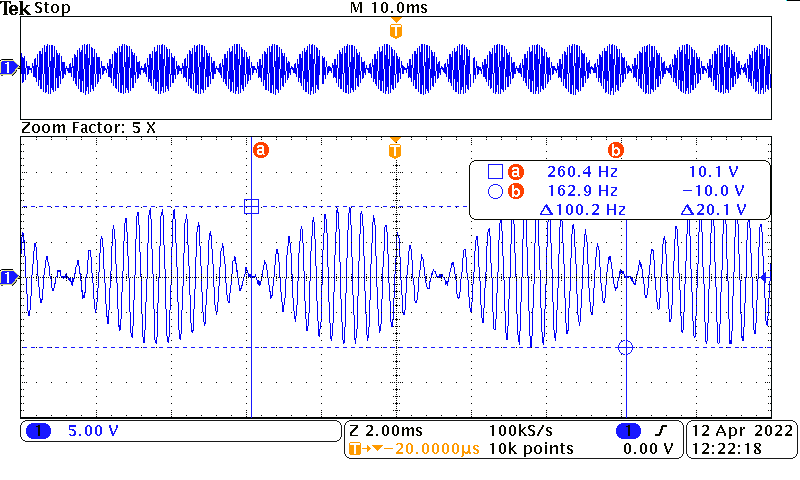
\includegraphics[width=\textwidth]{include/3/1.png}
    \caption{Przebieg napięcia wyjściowego \(U_{wy}\)}
\end{figure}
